\section{RQ2: Do Benchmarks Execute the Edited Code?}
\label{sec:rq2}

\paragraph*{Result}
On networkx, for \BOneAgentUnreached{} of the \NxAgentOpt{} replayed optimization edits (\BOneAgentPct\pct, Wilson CI \ci{\BOneAgentLo}{\BOneAgentHi}), the measured profile of no benchmark case contains any function the edit changed (Fig.~\ref{fig:coverage}).
By static reach, \BOneAgentStatic{} of \NxAgentOpt{} are unreached (\BOneAgentStaticPct\pct, \ci{\BOneAgentStaticLo}{\BOneAgentStaticHi}).
With the earlier subject-only labels the counts are \BOneManualUnreached{} of \NxManualOpt{} (\BOneManualPct\pct, \ci{\BOneManualLo}{\BOneManualHi}) by profile and \BOneManualStatic{} of \NxManualOpt{} by static reach; over all \NxReplayed{} replayed edits they are \BOneAllUnreached{} and \BOneAllStatic{}.
The two label sets differ by one edit, which is unreached under both measures, so the reading does not depend on the labels.
Because every interval includes values below one half, we say that \emph{many} optimization edits on networkx are unreached, not most.

\begin{figure}[t]
\centering
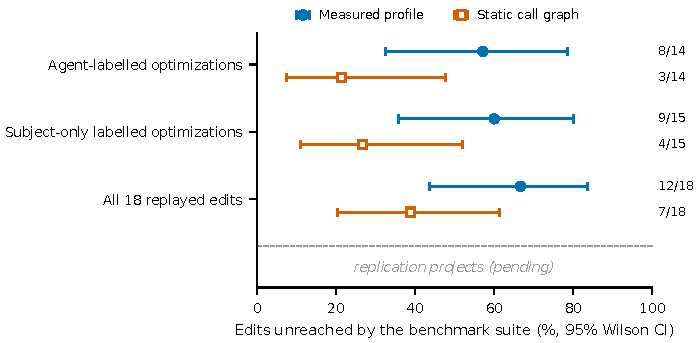
\includegraphics[width=\columnwidth]{figures/fig_coverage.pdf}
\caption{Share of replayed networkx edits that no benchmark executes, by measured profile and by static reach, with Wilson 95\pct{} intervals, for three edit sets. The replication rows are pending.}
\label{fig:coverage}
\end{figure}

\paragraph*{Reach at the base state}
Reach was measured with the $S_0$ suite and $S_0$ profiles.
An edit could be counted as unreached by construction if its changed functions did not exist at $S_0$.
We looked up every changed function of the labelled optimizations by qualified name at $S_0$ and at the edit's parent: \ConstructUnreached{} edits are unreached by construction.
Every one has at least one changed function that exists at $S_0$, and all changed functions exist at their parent; the only partial absence is a nested helper that step~2 adds inside \texttt{bidirectional\_dijkstra}, whose enclosing function exists at $S_0$ and is also absent from every $S_0$ profile.
The unreached count therefore stands.
What remains is that profiles were taken with the $S_0$ suite at $S_0$, not at each edit's parent; the replay excluded test and benchmark files, so a benchmark added upstream between $S_0$ and an edit would not be seen.
\TODO{Recompute the unreached count with the upstream suite and profiles at each edit's parent, as the replication protocol does; give the date span of the replayed commits.}

\TODO{E1 (B1 replication on 3--4 projects): per-project and pooled unreached share with Wilson CIs (forest plot rows in Fig.~\ref{fig:coverage}), measured profiles at each edit's parent, edits classified from the diff by two raters with $\kappa$; report attrition per the pre-registered rule. If the pooled share is low (the advisor's threshold: below a quarter), reframe RQ2 as ``coverage depends on suite design'' and lead with the coverage, share and power decomposition.}

\paragraph*{Static reach is not a bound}
Static reach leaves fewer edits unreached than the measured profile, on every edit set.
It over-approximates through module-level edges and import closure: the heavy benchmark module imports most of the package, so a static graph connects it to functions it never calls.
Static reach from an old base can also err the other way, by missing functions added after the base (Appendix~\ref{app:q3}).
A coverage study of optimization edits therefore needs measured profiles; static counts from one base bound nothing in either direction.

\paragraph*{Example}
The motivating edit (step~2, \texttt{bidirectional\_dijkstra}) is unreached by profile but reached by static reach, which connects all \NxBenchCases{} cases to it.
\TODO{Table 3: three to five unreached optimization edits (step, changed function, commit subject, nearest benchmark), generated from \texttt{labelling/precision\_b1.json} and the $S_0$ profile.}

\paragraph*{Suite design as a moderator}
The networkx suite is organized by graph class and algorithm family, with one module holding most algorithm benchmarks.
bottleneck's suite, by contrast, names its functions directly; we conjecture that its edits are mostly reached by name, but our static pilot cannot show it (Appendix~\ref{app:q3}). A source reading shows that even there, one benchmark of \texttt{nanmax} calls \texttt{nanmin}, so code specific to \texttt{nanmax} is never benchmarked.
Whether benchmarks see optimization edits thus depends on how the suite is written, which the replication must show across projects.

\paragraph*{Robustness}
A re-profile at $S_0$ in an isolated work tree reproduced the executed-function sets of all \ReprofileCases{} cases of the first profiling part, whose provenance had been disturbed (Appendix~\ref{app:lessons-detail}).
Profiles are from one call per case at one state; dependency data of this kind is partly nondeterministic (Section~\ref{sec:lessons}), so a profile is a sample of reach, not its complete set.

\paragraph*{Answer to RQ2}
On networkx, the project's own benchmarks do not execute the changed code of many optimization edits (\BOneAgentUnreached{} of \NxAgentOpt{}, CI \ci{\BOneAgentLo}{\BOneAgentHi}).
For those edits, even full benchmarking cannot confirm the speed-up or see a slowdown.
